Mobile applications have the potential of collecting massive amount of data from their users. This can be used to increase user experience but also lead to intrusive behaviour. Permissions is a great place to see if something is out of the ordinary. Some of the most interesting permissions related to privacy of the application:  

\begin{itemize}
    \item INTERNET \& ACCESS NETWORK STATE
    \item MANAGE ACCOUNTS \& GET ACCOUNTS \& USE CREDENTIALS
    \item ACCESS FINE LOCATION \& ACCESS COARSE LOCATION
\end{itemize}

The networking permissions are obviously necessary. The account permissions are used to authenticate with either Google or Facebook. The most interesting are the location related. When opening the application the user is prompted whether he will allow location tracking when using the app. This setting is persistent and can not be disabled from the application. The user has to disable it in settings. Additionally there should be an option to allow for one session. The location permission does not seem necessary for the application. The only use is related to a map shown on items for sale. As Google Maps is used for this feature it might be a needed permission.

The data collection of the application revolves around how users use the application and advertisement. Almost whenever button is pressed a chain of requests are performed. A chain can be seen on figure \ref{fig:statistics-chain}. 

\begin{figure}[htbp]
    \centering
    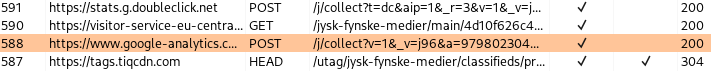
\includegraphics[width=1\columnwidth]{../static-analysis/pictures/statistics_trackview_chain.png}
    \caption{Analytics chain on user actions}
    \label{fig:statistics-chain}
\end{figure}

An example of the request can be seen on Figure \ref{fig:statistic-request-car}. This request is triggered by the car category when searching for items.  

\begin{figure}[htbp]
    \centering
    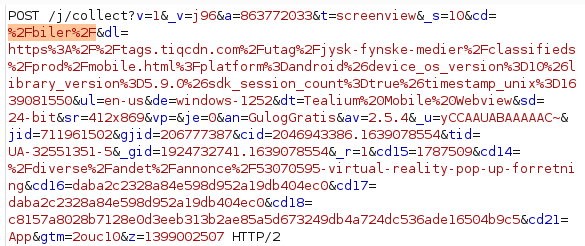
\includegraphics[width=1\columnwidth]{../dynamic-analysis/pictures/analytics-request-cars.png}
    \caption{Analytics request when pressed on the cars(biler) category}
    \label{fig:statistic-request-car}
\end{figure}

These requests send the user's actions to external services. It is seen that the event is sent to Google Analytics and Doubleclick. Doubleclick is an advertisement company owned by Google. This result in targeted advertisements for the user dependent on his behaviour in the application. There is a range of trackers. An overview can be seen on Table \ref{tab:trackers}. 

\begin{table}[]
    \centering
    \begin{tabular}{|l|l|l|}
    \hline
    \textbf{Company} & \textbf{Tracker Name} & \textbf{Category} \\ \hline
    Facebook         &                       &                   \\ \hline
                     & Ads                   & Advertisement     \\
                     & Analytics             & Analytics         \\
                     & Audience              & Analytics         \\ \hline
    Google           &                       &                   \\ \hline
                     & AdMob                 & Advertisement     \\
                     & Analytics             & Analytics         \\
                     & CrashLytics           & Crash reporting   \\
                     & DoubleClick           & Advertisement     \\ \hline
    Tealium          &                       & Analytics         \\ \hline
    \end{tabular}
    \caption{Overview of some of the trackers}
    \label{tab:trackers}
\end{table}

The analytics trackers are used to improve user experience. Looking at metrics regarding user sessions and actions. CrashLytics is used to report crashes and tell the developers the state of the application at the incident. The advertisement trackers are retrieving information from the users behaviour and thus targeting advertisements thereof. If the user authenticates with both Facebook and Google, it is expected that the tracking goes beyond the scope of this application. Meaning the behaviour of the user might be visual in ads he receives on other platforms. Other than that there is no integration to Social Networks.       